\section{Introduction}

Transformer-based language models~\cite{vaswani2017attention,Radford2018GPT,radford2019language,devlin2018bert, roberta,xlnet,T5} in Natural Language Processing (NLP) have driven rapid progress in recent years as computation at scale has become more available and datasets have become larger. Recent work~\cite{gpt3, shoeybi2019megatron} has shown large language models to be effective zero- or few-shot learners, with high accuracy on many NLP tasks and datasets. These large language models have a number of exciting downstream applications such as client feedback summarization, automatic dialogue generation, semantic search, and code autocompletion~\cite{gpt3applications, microsoftcodecompletion, githubcopilot}.
As a result, the number of parameters in state-of-the-art NLP models have grown at an exponential rate (Figure~\ref{fig:model_trend}). Training such models, however, is challenging for two reasons: (a) it is no longer possible to fit the parameters of these models in the main memory of even the largest GPU (NVIDIA recently released 80GB-A100 cards), and (b) even if we are able to fit the model in a single GPU (e.g., by swapping parameters between host and device memory~\cite{ren2021zero}), the high number of compute operations required can result in unrealistically long training times (e.g., training GPT-3 with 175 billion parameters~\cite{gpt3} would require approximately 288 years with a single V100 NVIDIA GPU). This calls for parallelism. Data-parallel scale-out usually works well, but suffers from two limitations: a) beyond a point, the per-GPU batch size becomes too small, reducing GPU utilization and increasing communication cost, and b) the maximum number of devices that can be used is the batch size, limiting the number of accelerators that can be used for training.

\begin{figure}[t!]
    \centering
    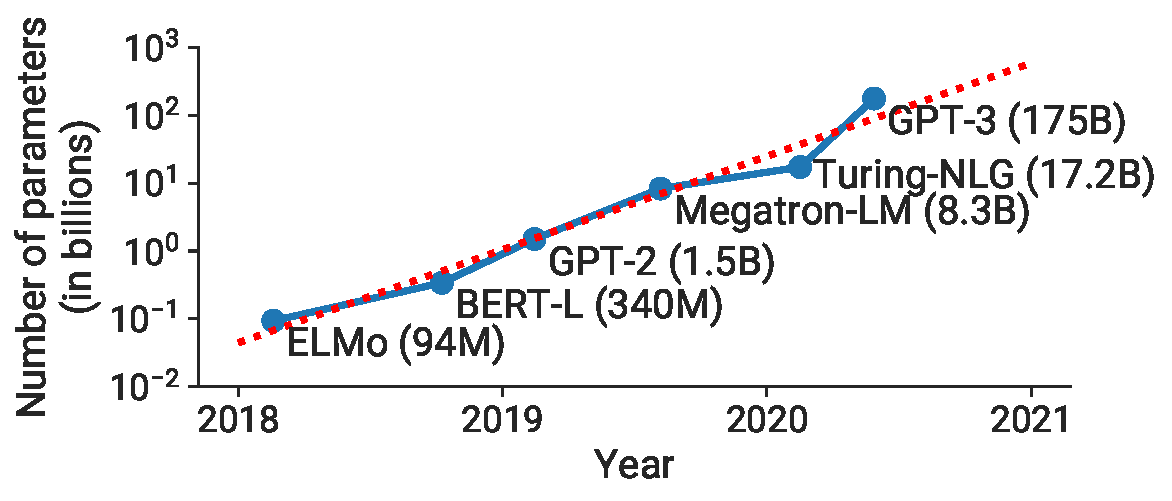
\includegraphics[keepaspectratio=1.0,width=0.95\columnwidth]{figures/model_trend.pdf}
    \vspace{-0.1in}
    \caption{
        Trend of sizes of state-of-the-art Natural Language Processing (NLP) models with time. The number of floating-point operations to train these models is increasing at an exponential rate.
    }
    \vspace{-0.1in}
    \label{fig:model_trend}
\end{figure}

Various model parallelism techniques have been proposed to address these two challenges. For example, recent work~\cite{mesh_tf,shoeybi2019megatron} has shown how tensor (intra-layer) model parallelism, where matrix multiplications within each transformer layer are split over multiple GPUs, can be used to overcome these limitations. Although this approach works well for models of sizes up to 20 billion parameters on NVIDIA DGX A100 servers (with 8 80GB-A100 GPUs), it breaks down for larger models. Larger models need to be split across multiple multi-GPU servers, which leads to two problems: (a) the all-reduce communication required for tensor parallelism needs to go through inter-server links, which are slower than the high-bandwidth NVLink~\cite{nvlink} available within a multi-GPU server, and (b) a high degree of model parallelism can create small matrix multiplications (GEMMs), potentially decreasing GPU utilization.

Pipeline model parallelism~\cite{narayanan2019pipedream, huang2019gpipe,narayanan2021memory, yang2021pipemare, pb2021kosson, fan2021dapple} is another technique to support the training of large models, where layers of a model are striped over multiple GPUs. A batch is split into smaller microbatches, and execution is pipelined across these microbatches. Layers can be assigned to workers in various ways, and various schedules for the forward and backward passes of inputs can be used. The layer assignment and scheduling strategy results in different performance tradeoffs. Regardless of schedule, to preserve strict optimizer semantics, optimizer steps need to be synchronized across devices, leading to a \emph{pipeline flush} at the end of every batch, where microbatches are allowed to complete execution (and no new microbatches are injected). As much as 50\% of time can be spent flushing the pipeline depending on the number of microbatches injected into the pipeline. The larger the ratio of number of microbatches to the pipeline size, the smaller the time spent in the pipeline flush. Therefore, to achieve high efficiency, a larger batch size is often necessary. In this work, we also introduce a new pipeline schedule that improves efficiency at small batch sizes.

Users can thus train their large models using various techniques, each with different tradeoffs. Moreover, these techniques can be \emph{combined}. However, combining these techniques leads to non-trivial interactions, which need to be reasoned through carefully for good performance. In this paper, we address the following question:
\begin{quote}
    \emph{How should parallelism techniques be combined to maximize the training throughput of large models given a batch size while retaining strict optimizer semantics?}
\end{quote}

In particular, we show how to combine pipeline, tensor, and data parallelism, a technique we call \emph{PTD-P}, to train large language models with good computational performance (52\% of peak device throughput) on 1000s of GPUs. Our method leverages the combination of pipeline parallelism across multi-GPU servers, tensor parallelism within a multi-GPU server, and data parallelism, to practically train models with a trillion parameters with graceful scaling in an optimized cluster environment with high-bandwidth links between GPUs on the same server and across servers. We can use similar ideas to train larger models as well, given more training resources. In our experiments, we demonstrate close to linear scaling to 3072 A100 GPUs, with an achieved end-to-end training throughput of 163 teraFLOP/s per GPU (including communication, data processing, and optimization), and an aggregate throughput of 502 petaFLOP/s, on a GPT model~\cite{gpt3} with a trillion parameters using mixed precision. This throughput facilitates practical training times: we estimate end-to-end training of this model to take $\sim 3$ months. We believe this is the fastest training throughput achieved for this size of model: past systems~\cite{shoeybi2019megatron, narayanan2019pipedream} cannot train such large models since they do not combine pipeline and tensor parallelism. We also compared to ZeRO~\cite{rajbhandari2019zero}, and found that our approach outperforms ZeRO-3 by $70\%$ for models with 175 and 530 billion parameters due to less cross-node communication. These models are too large to fit on a multi-GPU server.

Achieving this throughput at scale required innovation and careful engineering along multiple axes: efficient kernel implementations that allowed most of the computation to be compute-bound as opposed to memory-bound, smart partitioning of computation graphs over the devices to reduce the number of bytes sent over network links while also limiting device idle periods, domain-specific communication optimization, and fast hardware (state-of-the-art GPUs and high-bandwidth links between GPUs on the same and different servers). We are hopeful that our open-sourced software (available at \url{https://github.com/nvidia/megatron-lm}) will enable other groups to train large NLP models efficiently at scale. 

In addition, we studied the interaction between the various components affecting throughput, both empirically and analytically when possible. Based on these studies, we offer the following guiding principles on how to configure distributed training:
\begin{itemize}
    \item Different forms of parallelism interact in non-trivial ways: the parallelization strategy has an impact on the amount of communication, the compute efficiency with which kernels are executed, as well as the idle time workers spend waiting for computation due to pipeline flushes (pipeline bubbles). For example, in our experiments, we found that sub-optimal combinations of tensor and pipeline model parallelism can lead to up to 2$\times$ lower throughput, even with high-bandwidth network links between servers; tensor model parallelism is effective within a multi-GPU server, but pipeline model parallelism must be used for larger models.
    \item The schedule used for pipeline parallelism has an impact on the amount of communication, the pipeline bubble size, and memory used to store activations. We propose a novel interleaved schedule that can improve throughput by as much as 10\% compared to previously-proposed schedules~\cite{huang2019gpipe,narayanan2021memory} with comparable memory footprint.
    \item Values of hyperparameters such as microbatch size have an impact on the memory footprint, the arithmetic efficiency of kernels executed on the worker, and the pipeline bubble size. In our experiments, the optimal value of the microbatch size is problem-dependent and can increase throughput by 15\%.
    \item At scale, distributed training is communication-intensive. When training a trillion-parameter model on 3072 GPUs, our implementation used an effective bisection bandwidth of 892 GB/s for pipeline-parallel communication, and 13 TB/s for data-parallel communication. Using slower inter-node interconnects or more communication-intensive partitionings would hinder scaling performance.
\end{itemize}
We should note that we do not automatically explore the search space of parallelism strategies (such as FlexFlow~\cite{flexflow}, PipeDream~\cite{narayanan2019pipedream}, Tarnawski et al.~\cite{tarnawski2020efficient}, and DAPPLE~\cite{fan2021dapple}), but instead suggest heuristics (in \S\ref{sec:parallelization_dimensions}) that we found work well in practice.
